%
% Modified by Sameer Vijay
% Last Change: Wed Jul 27 2005 13:00 CEST
%
%%%%%%%%%%%%%%%%%%%%%%%%%%%%%%%%%%%%%%%%%%%%%%%%%%%%%%%%%%%%%%%%%%%%%%%%
%
% Sample Notre Dame Thesis/Dissertation
% Using Donald Peterson's ndthesis classfile
%
% Written by Jeff Squyres and Don Peterson
%
% Provided by the Information Technology Committee of
%   the Graduate Student Union
%   http://www.gsu.nd.edu/
%
% Nothing in this document is serious except the format.  :-)
%
% If you have any suggestions, comments, questions, please send e-mail
% to: ndthesis@gsu.nd.edu
%
%%%%%%%%%%%%%%%%%%%%%%%%%%%%%%%%%%%%%%%%%%%%%%%%%%%%%%%%%%%%%%%%%%%%%%%%

%
% Chapter 3
%

\chapter{TWO PROTON TRANSFER AT NOTRE DAME}
\label{chap:2pExpt}

\begin{comment}
Give an overview of the requirements for two-proton transfer and say that ND has a buncher and a Tandem accelerator that goes up to 10 MV so we can get beam energies up to 30 MeV for \He{3} and we have a beamline with a long flight path SO we can do this experiment.
\end{comment}

The previous chapter demonstrated the interest in studying \reaction reactions.  The detected reaction product is a neutron and its time of flight (TOF) must be measured.  The beam must therefore be bunched and the neutron detector must be optimized to provide excellent timing information.  The bunching of the beam and the timing properties of the neutron detector will be discussed in detail in this chapter.   

% detecting neutrons
% this means we need timing information
% so the beam must be bunched
% and the detector must be built to give good timing
% and placed to give good timing

% interested in 0+ distribution
% and there's an ideal beam energy for that
% and that constrains the distance between the target and neutron detector
Not only must the beam be bunched, its energy must also be carefully chosen.  As discussed in the previous chapter, the purpose of this experiment is to measure the distribution of \zp strength.  According to DWBA calculations, achieving the maximum \zp cross-section for \reaction requires a beam energy near 18 MeV, but the resolution of the neutron detector decreases with increasing neutron energy.  The energy chosen for the \He{3} is 16 MeV, and the effect of this energy on the resolution of the neutron detector is discussed in {\sect}~\ref{sec:detector}.


\section{Beam Production at Notre Dame}
\label{sec:beamProduction}

The beam delivered to the target is 16 MeV bunched \He{3}.  In this section, we will follow the beam through its production and acceleration.

The Helium Ion Source (HIS) provides negative \He{3} ions to the accelerator.  A duoplasmatron ion source filled with \He{3} gas uses a discharge across high voltage to convert some of the gas into plasma.  Electrostatic elements extract positive \He{3} ions from the plasma and accelerate them into a canal filled with lithium vapor.  Lithium is crucial for creating negatively charged beam because it donates electrons generously, and a small fraction of the \He{3} becomes negatively ionized after passing through the canal.  A dipole magnet after the ion source removes the carbon, oxygen, and other impurities that contaminate the \He{3} beam.  Movable, thick tungsten slits stop these contaminants and allow beam within a small range of magnetic rigidity (see {\eqn}~\ref{eqn:rigidity} below) to pass through to the accelerator.  Typically, the maximum output of the HIS is $\sim$1~$\mu$A.

The accelerator at Notre Dame is a tandem Van de Graaff accelerator made by High Voltage Engineering Corporation.  Its maximum terminal potential is 10~MV.  Negatively charged beam enters and accelerates toward the positive terminal, located in the center of the machine. A thin carbon foil ($\sim$ 3 $\mu$g/cm$^2$) in the center of the machine strips electrons from the beam.  The now-positive beam accelerates again, away from the positive terminal. In general, the final energy of a particular beam is then

\begin{equation}
E_{\text{beam}} = E_{\text{HIS}} + (1+q)eV_{\text{T}},
\label{eqn:beamEnergy}
\end{equation}
where $V_{\text{T}}$ is the terminal voltage, $E_{\text{HIS}}$ is the energy of the beam exiting the HIS, $q$ is the charge state of the beam after passing through the carbon foil, and $e$ is the charge on the electron.  \He{3} beam is fully stripped of its electrons by the carbon foil, and so the terminal voltage required to produce 16 MeV \He{3} is 5.33~MV, well within the operating voltage range of the accelerator.    

A dipole magnet with a magnetic field strength $B$ will bend a particle with momentum $p$ and charge $qe$ in a circle of radius $R$.  The product of the field strength and the radius of the path, $BR$, is called the magnetic rigidity, and is proportional to the ratio of the momentum and the charge of a particle:

\begin{equation}
BR = \frac{p}{qe} = \frac{\sqrt{2mE}}{qe}.
\label{eqn:rigidity}
\end{equation}

A large 90$^{\circ}$ bend dipole magnet at the exit of the tandem can work in a feed-back circuit to regulate the terminal voltage.  Since the mass and charge of the desired beam are fixed, selecting beam at a fixed radius exiting a dipole defines its energy.  Horizontal slits at the dipole entrance and exit are approximately one millimeter apart.  Both sets of slits serve to narrowly define the beam, but the slits after the analyzing magnet each read the current from incident beam.  This slit current is a sensitive measure of the terminal voltage and is used in a feed-back circuit to maintain a constant beam energy.  Since the radius of the dipole magnet is one meter, the momentum is defined to one part in 1000 and the energy to two parts in 1000 for a fixed magnetic field.  If the terminal voltage drifts up or down, the beam energy will change with it and the beam trajectory will travel a larger or smaller radius through the dipole.  For \He{3}, $E_{\text{beam}}\sim3V_{\text{T}}$, and so a change in the terminal voltage of even one part in 1000 will alter the balance of the slit current.  Because this regulation is limited by the stability of the magnetic field of the dipole, the analyzing magnet is calibrated against the nuclear magnetic resonance (NMR) of hydrogen.  Using it to regulate the terminal voltage reduces the ripple in the voltage to approximately 10~kV.


\subsection{Beam Focusing and Selection}

Beam exiting the analyzing magnet is narrowly defined by horizontal and vertical slits.  Additionally, both pole faces of the analyzing magnet are shaped to provide a focusing field in both the horizontal and vertical planes.  Although the beam has a limited angular divergence at the analyzing magnet, the flight path to the target is $\sim60$~m and and many focusing and steering elements along the way are necessary to obtain a reasonable transmission rate and ensure that the beam is well-focused at the target.  See {\fig}~\ref{fig:beamline} for a schematic diagram of the focusing and steering elements along the beamline.  Two Einzel lenses \citep{BeamOptics} focus the beam before it enters the accelerator, and a set of electrostatic steerers before and after the accelerator are enough to position the beam before it enters the analyzing magnet.  Quadrupole doublet magnets focus the beam as it travels through the target rooms, and another set of steerers allows correction of the beam position and angle.  The final focusing elements before the target are two large-bore, variable-strength solenoid magnets \citep{TwinSol} that focus the beam to a spot approximately 2~mm in diameter.

% figure: beamline
\begin{figure}[htp]
\centering
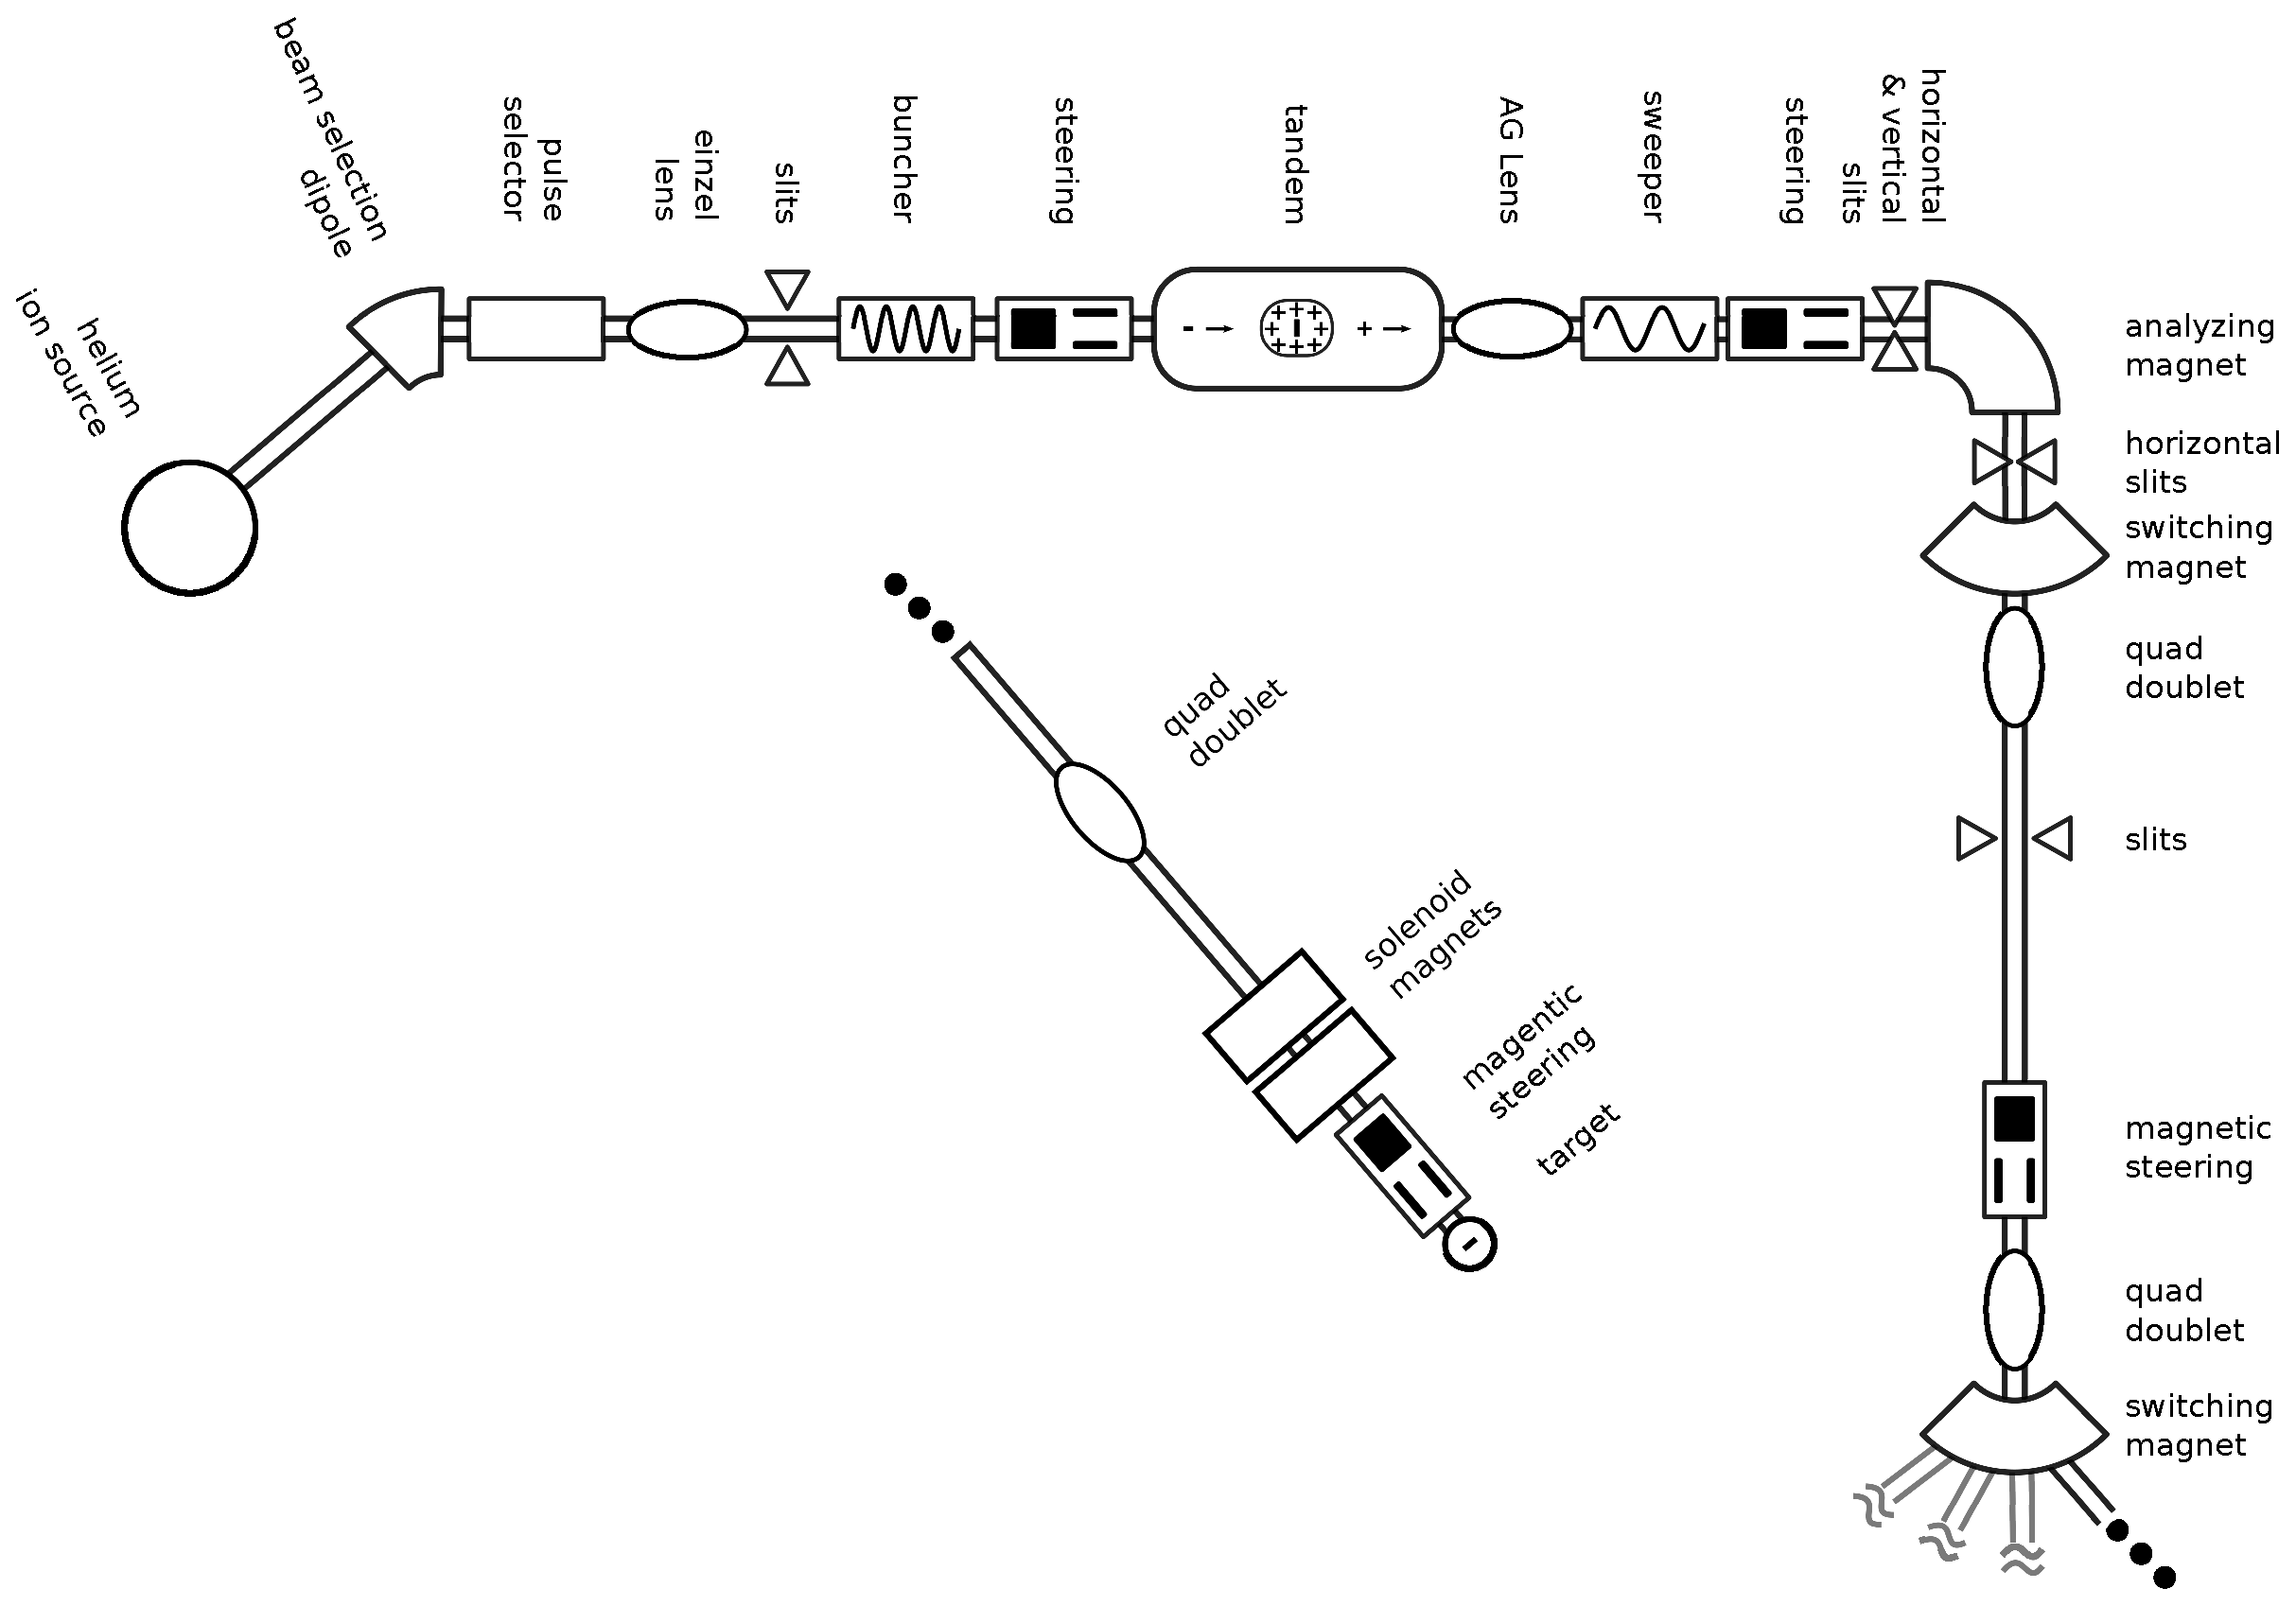
\includegraphics[width=1.0\textwidth]{figures/NSL_beamline.eps}
\caption[Beam production at Notre Dame.]{Beam production at Notre Dame.  The center inset shows the 15$^{\circ}$ beamline that was used in the experiments.}
\label{fig:beamline}
\end{figure}

\subsection{Beam Bunching}

Continuous beam would make it impossible for our detector to determine the neutron TOF.  It is possible to bunch the beam so that ``bunches'' of \He{3} arrive at the target, each bunch having a time spread of approximately one ns. There are three components to the bunching system at Notre Dame.  The first is the buncher itself, which pushes about 40\% of the beam into discrete bunches.  The remaining 60\% is a continuous background and must be removed with the ``sweeper''.  Together, the buncher and sweeper provide bunches of beam that are 1 ns wide at the target and separated by 101 ns, with no beam in between.  With the detector approximately 15 m away from the target, some of the slow neutrons coming from the reaction have a TOF in excess of 300 ns.  A pulse-selector is used to eliminate three out of every four bunches to avoid overlapping energetic neutrons from the current beam bunch with slow neutrons from the previous bunch.  The buncher, sweeper, and pulse-selector together provide clean bunches of beam separated by 400 ns.  The rest of this section describes how each of these components works.

The beam buncher operates by slowing down particles that would arrive too early at the target and speeding up particles that would be arriving too late.  To achieve this, two grids perpendicular to the beam connect to a radio-frequency (RF) power supply to create a time-varying electric field.  If the electric field were a sawtooth wave in time, the beam bunches would contain all the beam \citep{LynchBunching}.  As illustrated in {\fig}~\ref{fig:bunching}, the buncher decelerates the early portion of the beam and accelerates the late portion of the beam.  The strength of the field determines the distance at which the bunch will be narrowest, with a stronger field bringing the bunch into time focus earlier than a weaker field.  The pure sawtooth field is able to bunch 100\% of the incoming beam because it immediately resets after its linear portion.  Commercially available RF power supplies, however, generally vary sinusoidally in time.  At Notre Dame, a single frequency buncher that operates at 9.85 MHz is used.  While the RF signal is increasing approximately linearly with time, beam is bunched exactly as if the field were a pure sawtooth wave.  When the electric field approaches a maximum or minimum, little bunching occurs, and when the electric field is decreasing, de-bunching occurs.  The sinusoidal RF supply results in nanosecond wide bunches containing $\sim$40\% of the beam arriving at the target every 101~ns, superimposed on a continuous background of the remaining beam.  This continuous beam would render our time signal useless and must somehow be removed.

% figure: how a beam buncher works
\begin{figure}[htp]
\centering
\includegraphics[width=1.0\textwidth]{figures/beamBunching.eps}
\caption[Beam bunching.]{Beam bunching using a time-varying electric field.  Each dot represents a beam particle, and the vertical gray bars represent the bunching electrodes.  To bunch one section of beam, particles arriving first must be slowed down, while particles arriving last must be sped up.  A linearly increasing field does exactly this.  If the wave is a perfect sawtooth, there is no time during which beam is not being bunched - that is, all the beam is bunched.  Notice also that beam does not exit the buncher in a tight bunch; as time passes, beam drifts together.  The time until the bunch is at its narrowest depends on the amplitude of the electric field applied by the buncher.}
\label{fig:bunching}
\end{figure}

The ``sweeper'' provides a sinusoidal electric field that is timed to deflect the continuous beam between the bunches.  A set of vertical slits immediately after the sweeper removes the deflected beam.  Variable delays allow adjustment of the timing between the buncher and the sweeper and must be optimized for a particular beam.  Even a few-nanosecond change in the timing can affect which portion of the beam is swept away. 

%figure of beam profile and sweeper

It is possible to take data without pulse selection.  However, the spread in TOF of the neutron spectrum is in excess of 300~ns, which complicates the TOF spectrum considerably.  With bunches arriving at the target every 101~ns, it will be impossible to tell if a neutron is very fast and associated with the current bunch or very slow and associated with the previous bunch.  The resulting spectrum is shown in Figure \ref{fig:PSvsNPS_TOF}.

% figure: the considerably complicated spectrum
\begin{figure}[htp]
\centering
\subfloat[][]{
   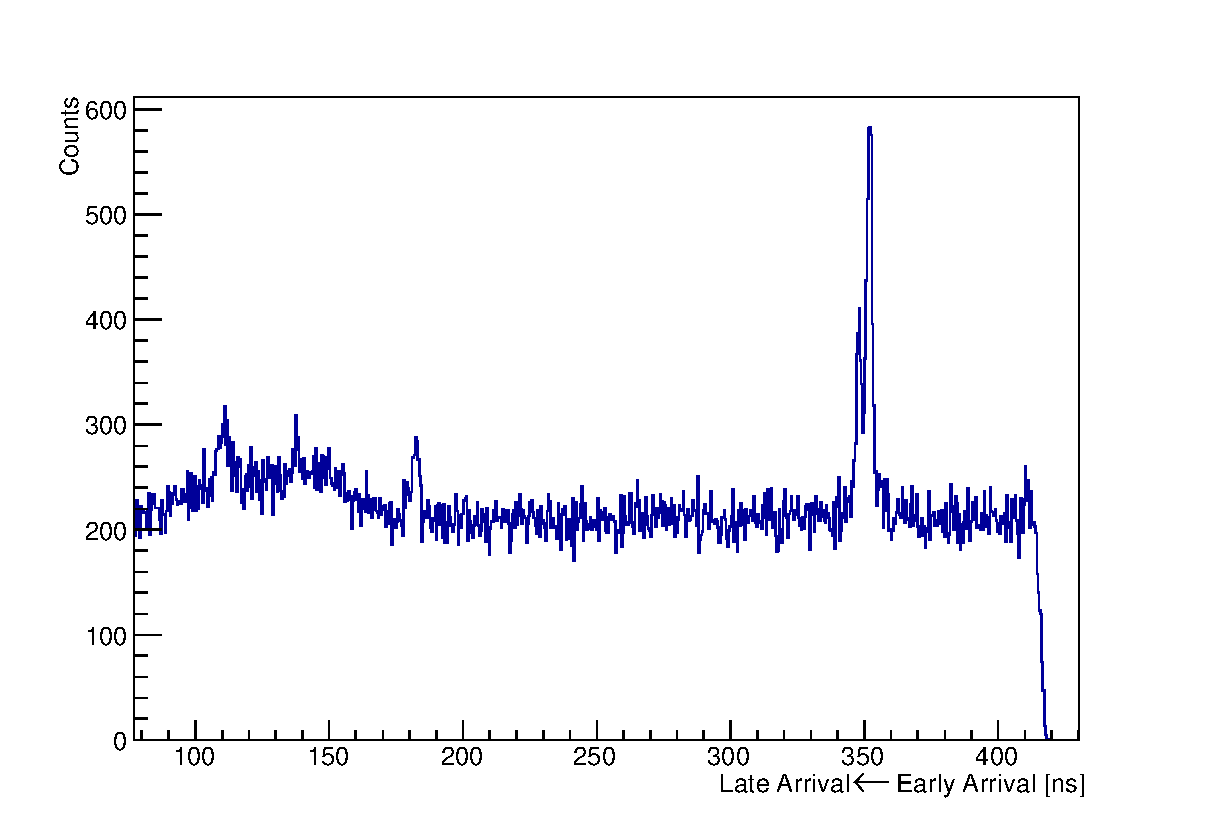
\includegraphics[width=0.45\textwidth]{figures/PS_BarA_Sep.eps}	
}
\subfloat[][]{
	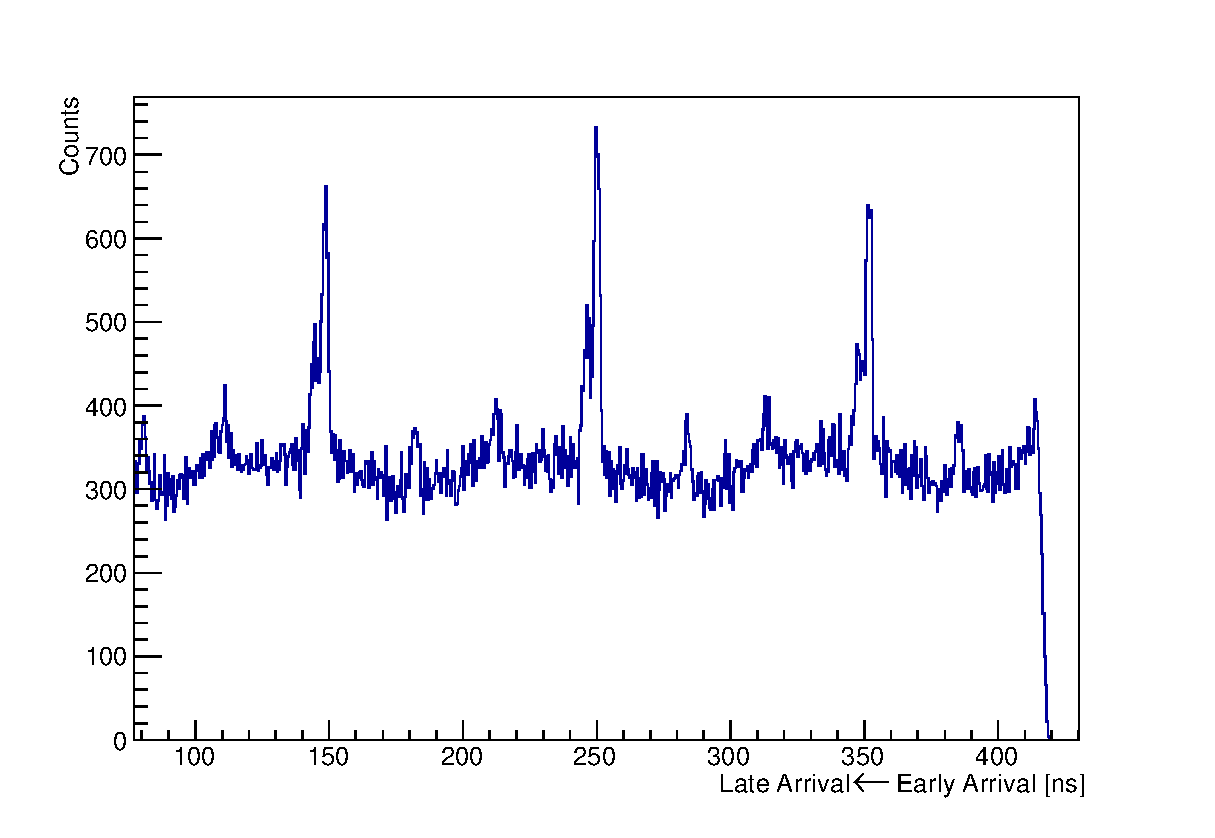
\includegraphics[width=0.45\textwidth]{figures/NPS_BarA.eps}
}
\caption[Timing spectra due to pulse-selected and non-pulse-selected beam.]{The timing spectrum from a pulse-selected beam is shown in (a).  The timing spectrum in (b) is from beam with no pulse selection.  Both timing spectra are from a \He{3} beam on a \Ge{76} target.  The constant background present in both images is due to random background radiation, not the beam.}
\label{fig:PSvsNPS_TOF}
\end{figure}

To give all the neutrons resulting from one beam bunch time to reach the detector before the next bunch strikes, a ``pulse selector'' eliminates three of every four bunches, resulting in 404~ns between each bunch at the cost of beam intensity.  The pulse selector is located before the accelerator and consists of two parallel plates, one held at ground and the other at +400 V.  A fast switch (SCR) connects the high-voltage plate to ground, letting the selected bunch through without deflection.  Vertical slits immediately after the pulse selector remove deflected beam, while undeflected beam passes through to the accelerator.  While the beam width is only one ns at the target, at the sweeper the bunch is approximately 80~ns wide, so the SCR must hold the plate at ground for 80~ns to let the entire bunch through.
% figure: slow neutrons and their dissappearance

Beam bunching and pulse selection reduce available beam current - the swept beam current is only 40\% $\times$ $\frac{1}{4} = 10$\% of the non-bunched current.  However, without bunched beam it would not be possible to distinguish the neutrons of interest in the (\He{3},n) transfer reaction.  Increased beam current would improve statistics on \reaction, but the HIS was already operating at its full output for these experiments.

\section{The Target Chamber}
\begin{comment}
target
thin stainless steel wall
Si detector
BaF$_2$ detector
\end{comment}

The 16 MeV \He{3} beam has been bunched, swept, pulse-selected, and steered and focused onto the target.  The bunches that were 80~ns wide before the accelerator have converged into 1-ns wide bunches at the target.  The target is at the center of a 2-mm thick stainless steel chamber that has a small gold-lined Faraday cup as shown in {\fig}~\ref{fig:targetChamber}.

To measure the absolute scale of the cross-section, it is necessary to know the number of particles incident on the target.  The charge measured by the Faraday cup is directly proportional to this number.  Additional detectors sensitive to the product of the beam current and the target thickness monitor the beam and provide relative normalization.  One of these is a Si detector placed inside the target chamber, which monitors \He{3} beam scattered from the target.  The other monitor detector is a BaF$_2$ detector located just outside the chamber.  It is sensitive to $\gamma$ radiation produced by beam interactions in the target.  
% figure: the target chamber & its detectors
\begin{figure}[htp]
\centering
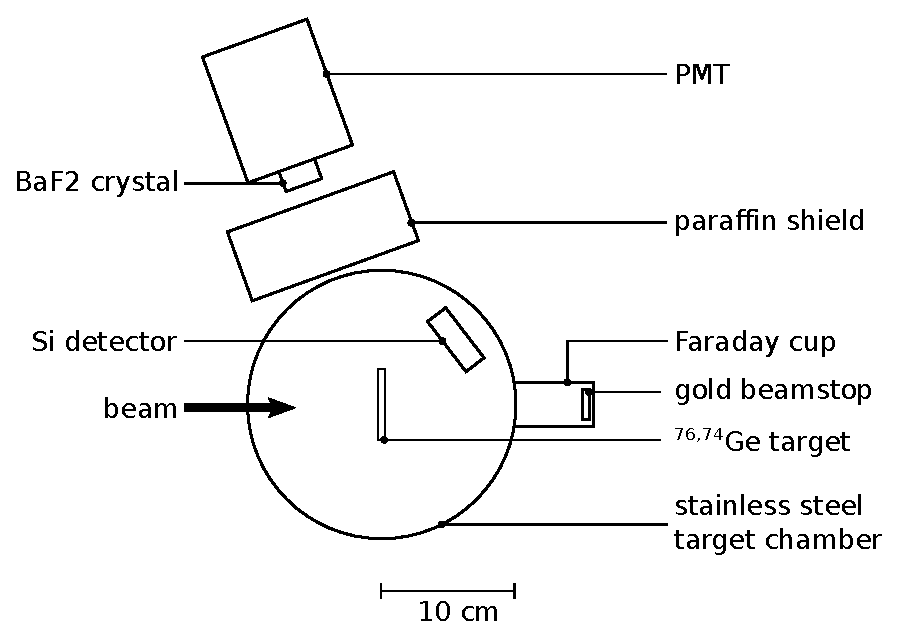
\includegraphics[width=1.0\textwidth]{figures/targetChamber.eps}
\caption[The target chamber and beam monitors.]{The target chamber and beam monitors.  The Si detector detects scattered \He{3} ions while the BaF$_2$ crystal primarily detects $\gamma$ radiation from the target.  Note that a paraffin block shields the BaF$_2$ detector from neutron radiation, which also escapes the target chamber.}
\label{fig:targetChamber}
\end{figure}


\section{The Neutron Detector}
\label{sec:detector}
\begin{comment}
Discuss neutron wall briefly.  Can reference NIMA paper. Explain why it's important that it's wide-angle. 
\end{comment}

The products of two-proton transfer onto \GeTargets are a neutron and a \SeProducts nucleus.  The neutron, lacking charge, is not likely to interact with remaining material in the target and has only a $\sim$5\% chance of scattering from the stainless steel target chamber.  This low rate of interaction, however, poses a challenge when the goal is to detect the neutron.  The neutron detector at Notre Dame maximizes the chance of a neutron interaction by providing protons with which the neutrons can strongly interact.  Unlike charged particles, neutrons rarely deposit their full energy in a detector.  Neutrons can only deposit all their energy when they collide head-on with a proton.  Much more likely is a glancing interaction, where the neutron imparts only some of its energy to the proton.  The measured energy spectrum of monoenergetic neutrons ranges from the detector threshold up to the neutron's full energy, making it impossible to determine the energy of the neutron from its deposited energy.  Instead, the time of flight (TOF) between the target and the detector is used to distinguish neutrons of differing energies.  The neutron detector is optimized to provide precise timing information.       
% figure of charged-particle energy spectrum
% figure of neutron energy spectrum

The neutron detector \citep{KolataNeutwall} consists of 16 large (1.5 m $\times$ 0.15 m $\times$ 0.05 m) bars of commercially available scintillator with excellent timing response \citep{BC408}.  Each plastic scintillator bar is equipped with two fast-risetime photomultiplier tubes (PMT's) at opposite ends.  The signal risetimes are approximately 5~ns, and by processing the signal with constant fraction discriminators (CFD's) the timing resolution of the PMT's is sub-nanosecond.  Additionally, PMT's on opposite ends of the bars allows construction of an average time signal, removing the timing spread due to the interaction location.  Neutron detector signal processing is discussed further in {\sect}~\ref{sec:electronics}.
% figure: one bar with its PMT's

% table: BC408 properties
\begin{table}[htp]
\centering
\caption[\uppercase{plastic scintillator properties}]{\uppercase{plastic scintillator properties}}
\label{tab:BC408}
\begin{tabular}{ll}
Properties & BC408 \\
\hline
Light Output, \% Anthracene & 64 \\
Rise Time, ns & 0.9 \\
Decay Time, ns & 2.1 \\
Pulse Width, FWHM, ns & $\sim2.5$ \\
Light Attenuation Length, cm & 210 \\
Wavelength of Max. Emission, nm & 425 \\
No. of H Atoms per cm$^3$ & 5.23$\times10^{22}$ \\
No. of C Atoms per cm$^3$ & 4.74$\times10^{22}$ \\
Ratio H:C Atoms & 1.104 \\
No. of Electrons per cm$^3$ & 3.37$\times10^{22}$ \\
\end{tabular}
\begin{flushleft}
\small NOTE:
Properties of the plastic scintillator used as the neutron detector. Values are taken from \citep{BC408}.
\end{flushleft}
\end{table}

The bars of scintillating plastic are positioned on an arc of radius 14.6 m centered around the target as shown in {\fig}~\ref{fig:detectorGeometry}.   At this distance, the solid angle subtended by each bar is only 0.15 m/15 m $\times$ 1.5 m/15 m = 1 msr.  The forwardmost angle relative to the beam is 6$^{\circ}$ and the largest angle is $22^{\circ}$.  As discussed in the previous chapter, the angular distribution of the \zp states peaks at 0$^{\circ}$ and drops to its first minimum at 20$^{\circ}$, so that ideally the detector would extend to 0$^{\circ}$.  A concrete support beam makes 6$^{\circ}$ the forwardmost instrumentable angle.
% figure - diagram of detector
\floatsetup[figure]{style=plain,subcapbesideposition=top}
\begin{figure}[htp]
\centering
\sidesubfloat[][]{
   
\includegraphics[width=1.0\textwidth]{figures/detectorLayout.eps}
}
\qquad
\sidesubfloat[][]{  
   
\includegraphics[width=0.35\textwidth]{figures/neutDetector_groupOfFour_crop.eps}
}
\caption[A schematic of the neutron detector and its supporting structure.]{A schematic of the neutron detector is shown in (a).  The figure is not to scale.  The detector is comprised of 16 independent scintillating bars, grouped in fours on separate support structures.  One of the supports is shown in (b).  Each individual bar of scintillator has a PMT fastened to its top and bottom surface.}
\label{fig:detectorGeometry}
\end{figure}

The 14.6~m flight path was not arbitrarily chosen; the distance between the target and detector must be as long as possible to ensure reasonable resolution.  The longest available path in the room was $\sim$15~m.  Together with the neutron energy, this distance determines the resolution of the detector.  Conservation of energy and momentum determines the relativistic energy $E = \gamma m c^2$ of the outgoing neutron, where $\gamma=(1-v^2/c^2)^{-1/2}$ and $m$ and $v$ are the rest mass and velocity of the neutron, respectively.  The time $t$ it takes for this neutron to travel the distance $d$ between the target and the detector is fixed for a given $d$ and $v$.  Deriving this time as a function of the relativistic energy is simple using the relation $E=\gamma mc^2$, where $c$ is the speed of light:
\begin{equation}
t(E) = \frac{d}{v} =  dc\times\sqrt{\frac{(E/mc^2)^2}{(E/mc^2)^2-1}} 
\label{eq:TOF}
\end{equation}
Neutrons from $^{76}$Ge($^3$He,n)$^{78}$Se have a relativistic energy of $\sim$966~MeV if the product nucleus, $^{78}$Se, is populated in its ground state.  Using {\eqn}~\ref{eq:TOF}, this gives a TOF of
\begin{eqnarray}
t(966 \text{ MeV}) &=& (14.6 \text{ m})(0.3 \text{ m/ns})\times\sqrt{\frac{(966/940)^2-1}{(966/940)^2}} \nonumber \\
           &=& (14.6 \text{ m})(0.3 \text{ m/ns})\times\frac{1}{0.23} = 212 \text{ ns} \nonumber.
\end{eqnarray}
Neutrons from a reaction that populates the first excited state of \Se{78}, which is only 0.6~MeV above the ground state, trail the ground-state neutrons by 1.9~ns.  Since the beam bunch itself has a width of 1~ns, this flight path provides not quite enough resolution to separate the ground and first excited state of \GeTargets. However, the differing angular distributions of the two states allowed for a determination of their respective intensities.  This is discussed in {\chap}~\ref{chap:dataAnalysis}.
% figure: \Ge{76}, 74Ge level scheme?


\subsection{Electronics}
\label{sec:electronics}
\begin{comment}
Electronics diagram!  Discuss two most important aspects: TDC and ADC from phototubes
\end{comment}

In principle, the timing information is all the data acquisition (DAQ) needs to record if there were no background radiation.  However, concrete in the room emits low-energy $\gamma$ radiation that leaves signals in the detector at a high rate.  Measuring the energy deposition is necessary because it allows us to eliminate this low-energy background radiation as well as high-energy cosmic rays.

When a particle deposits energy in some bar of the neutron detector, the DAQ must record both the total energy and timing of the signals from the top and bottom PMT's.  A charge to digital converter (QDC) can integrate the PMT signal and a time to digital converter (TDC) can measure the time between a logic pulse created by the PMT signal and the logic pulse from the beam buncher.  Because time resolution is the only way to distinguish groups of neutrons with different energies, constant fraction discriminators (CFD's) and not leading edge discriminators create the logic pulse sent to the TDC.  The 5-ns PMT signal risetime, together with CFD's, give timing information with jitter that is about 1~ns.  There are no stringent requirements on energy resolution as the detector itself has energy resolution on the order of 1~MeV near the thorium edge.
% figure: CFD operation

The lone signal provided by the PMT base is not adequate for pulse processing because the QDC and TDC require separate signals.  The signal from the PMT base is also too small to trigger the CFD's.  A 10$\times$ amplifier makes the signal large enough to trigger the CFD's and provides two copies of the input signal, one which can be analyzed for timing information while the other is analyzed for energy information.  A simplified diagram of the data acquisition is shown in {\fig}~\ref{fig:simpleElectronics}.

% figure: simple electronics
\begin{figure}[htp]
\centering
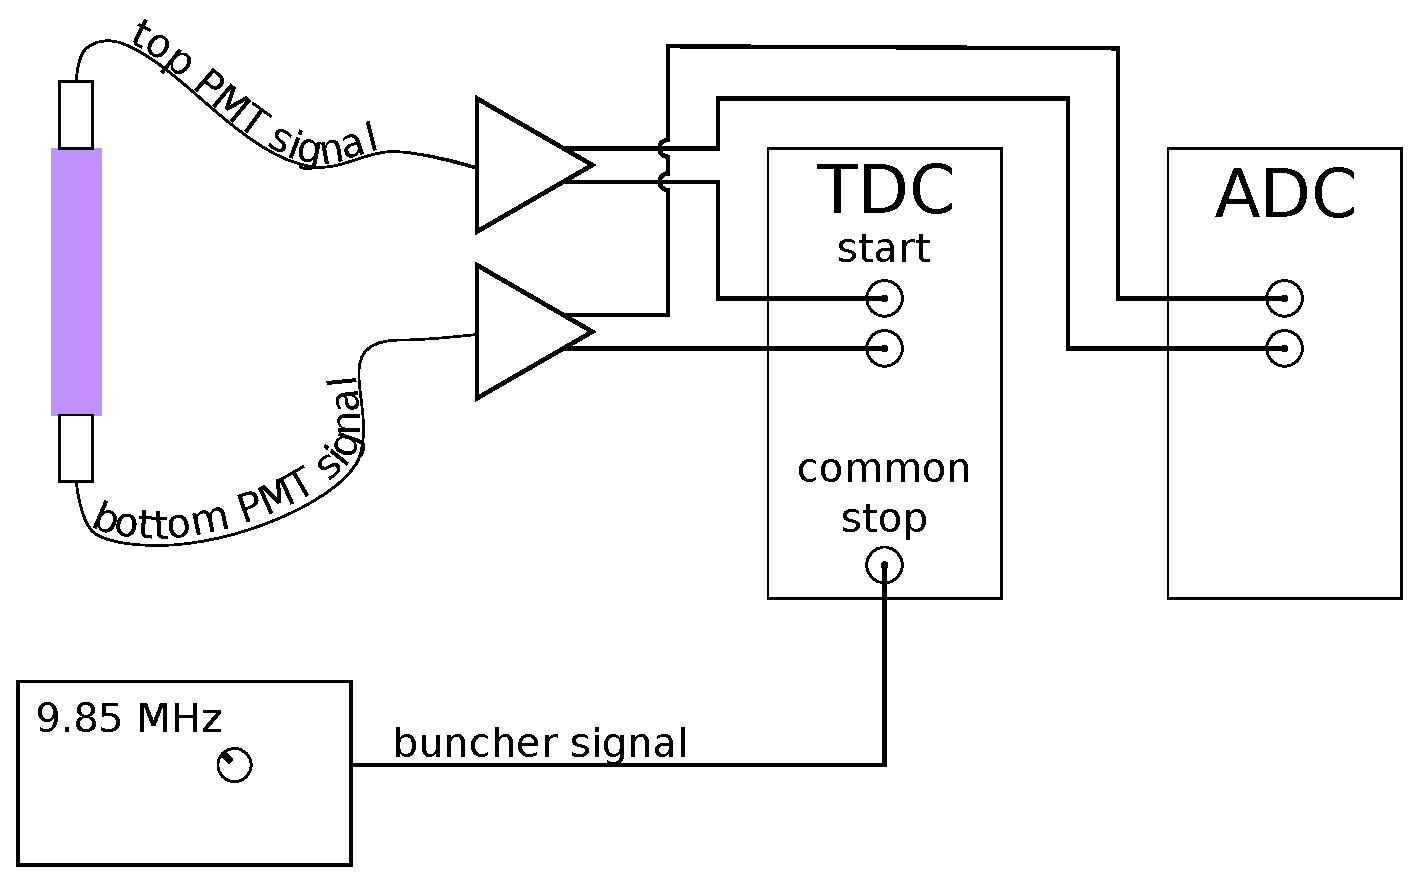
\includegraphics[width=1.0\textwidth]{figures/basic_electronics.eps}
\caption[Simplified sketch of the detector electronics.]{A simplified diagram of the neutron detector electronics showing the acquisition of timing and energy information from a single bar of the detector.}
\label{fig:simpleElectronics}
\end{figure}

The fundamental components of the DAQ are the TDC, the QDC, and the event trigger that causes the DAQ to read each module.  Triggering any time either a bar's top or bottom PMT fired would waste the DAQ with recording many noise events.  A real event should create signals in both the top and bottom PMT's, and requiring a coincidence between the two results is a reasonable trigger.  One way to define an event trigger for the entire neutron wall would be to trigger any time a coincidence between associated top and bottom PMT's occurs.  But constructing this trigger with NIM logic units requires many separate logic gates and is unnecessarily complicated.  

One solution is to use the built-in OR of the CFD.  Each CFD is an eight-fold unit that provides an OR output.  Instead of requiring a top and bottom signal in the same bar, each CFD unit processes a section of only top or only bottom bar signals and the condition is loosened to requiring a signal in a top PMT and a bottom PMT in the same eight-bar group as shown in {\fig}~\ref{fig:eventTrig}.  The presence of some top signal AND some bottom signal triggers the event signal.  Such an event only requires that both a top and a bottom signal coincided but does not require that these signals belonged to the same bar.  This simplified event trigger includes all events of interest, where the top and bottom signal belong to one bar, but also includes spurious events where no bar has a signal in both its top and bottom PMT.  With a dead time of less than 30\%, this event condition does not hinder data collection.  Simple software cuts eliminate any spurious events where no bar has a signal in both its top and bottom PMT.

% figure: event trigger
\begin{figure}[htp]
\centering
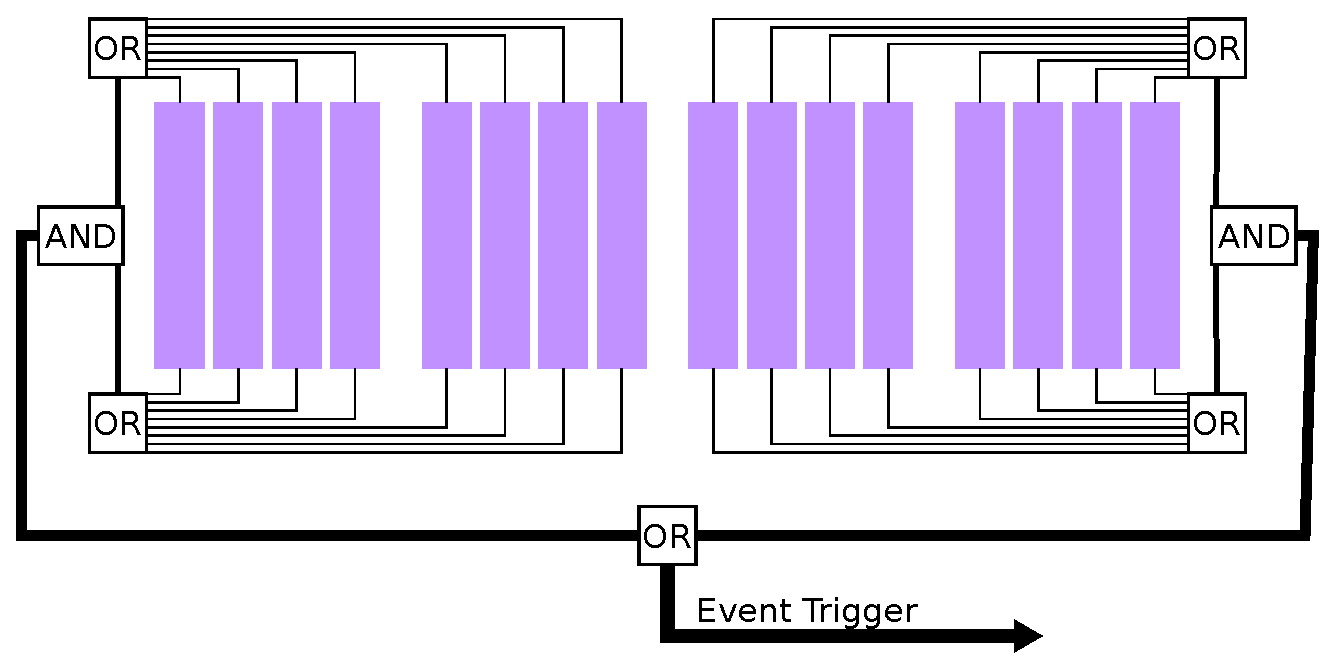
\includegraphics[width=1.0\textwidth]{figures/event_trigger.eps}
\caption[DAQ event trigger.]{The event trigger for the DAQ requires a coincidence between a top PMT and a bottom PMT from the same group of eight bars.}
\label{fig:eventTrig}
\end{figure}

% discuss energy, time info from near-target detectors
% and then scalers?
The time information, energy information, and a signal to indicate that this information should be read from the modules and recorded, form the core of the neutron detector DAQ.  However, the DAQ must also record information from the detectors near the target.  The particles of interest for the Si detector are scattered \He{3} beam, and because they are charged and deposit all their energy in the Si detector, the energy is a useful way to identify scattered \He{3} and should be recorded.  The BaF$_2$ detector sits outside the target chamber and monitors primarily beam-induced $\gamma$ radiation.  The timing of this detector's signal relative to the beam buncher, rather than the energy, is recorded by the DAQ.  Finally, because these detectors have high detection efficiency and are placed close to the target, their event rate is much higher than that of the neutron detectors.  While these detectors are essential to determining the relative particle flux through the target, the dead time they cause the DAQ should not prohibit events from the neutron detector itself from being recorded.  Pre-scaling the signals from the Si and BaF$_2$ by factors of 100 and 50, respectively, before adding it to the event trigger limits the dead time of the total system to less than 20\%.  See {\fig}~\ref{fig:fullElectronics} for a schematic of the complete electronics setup.
% figure: full electronics
\begin{figure}[htp]
\centering
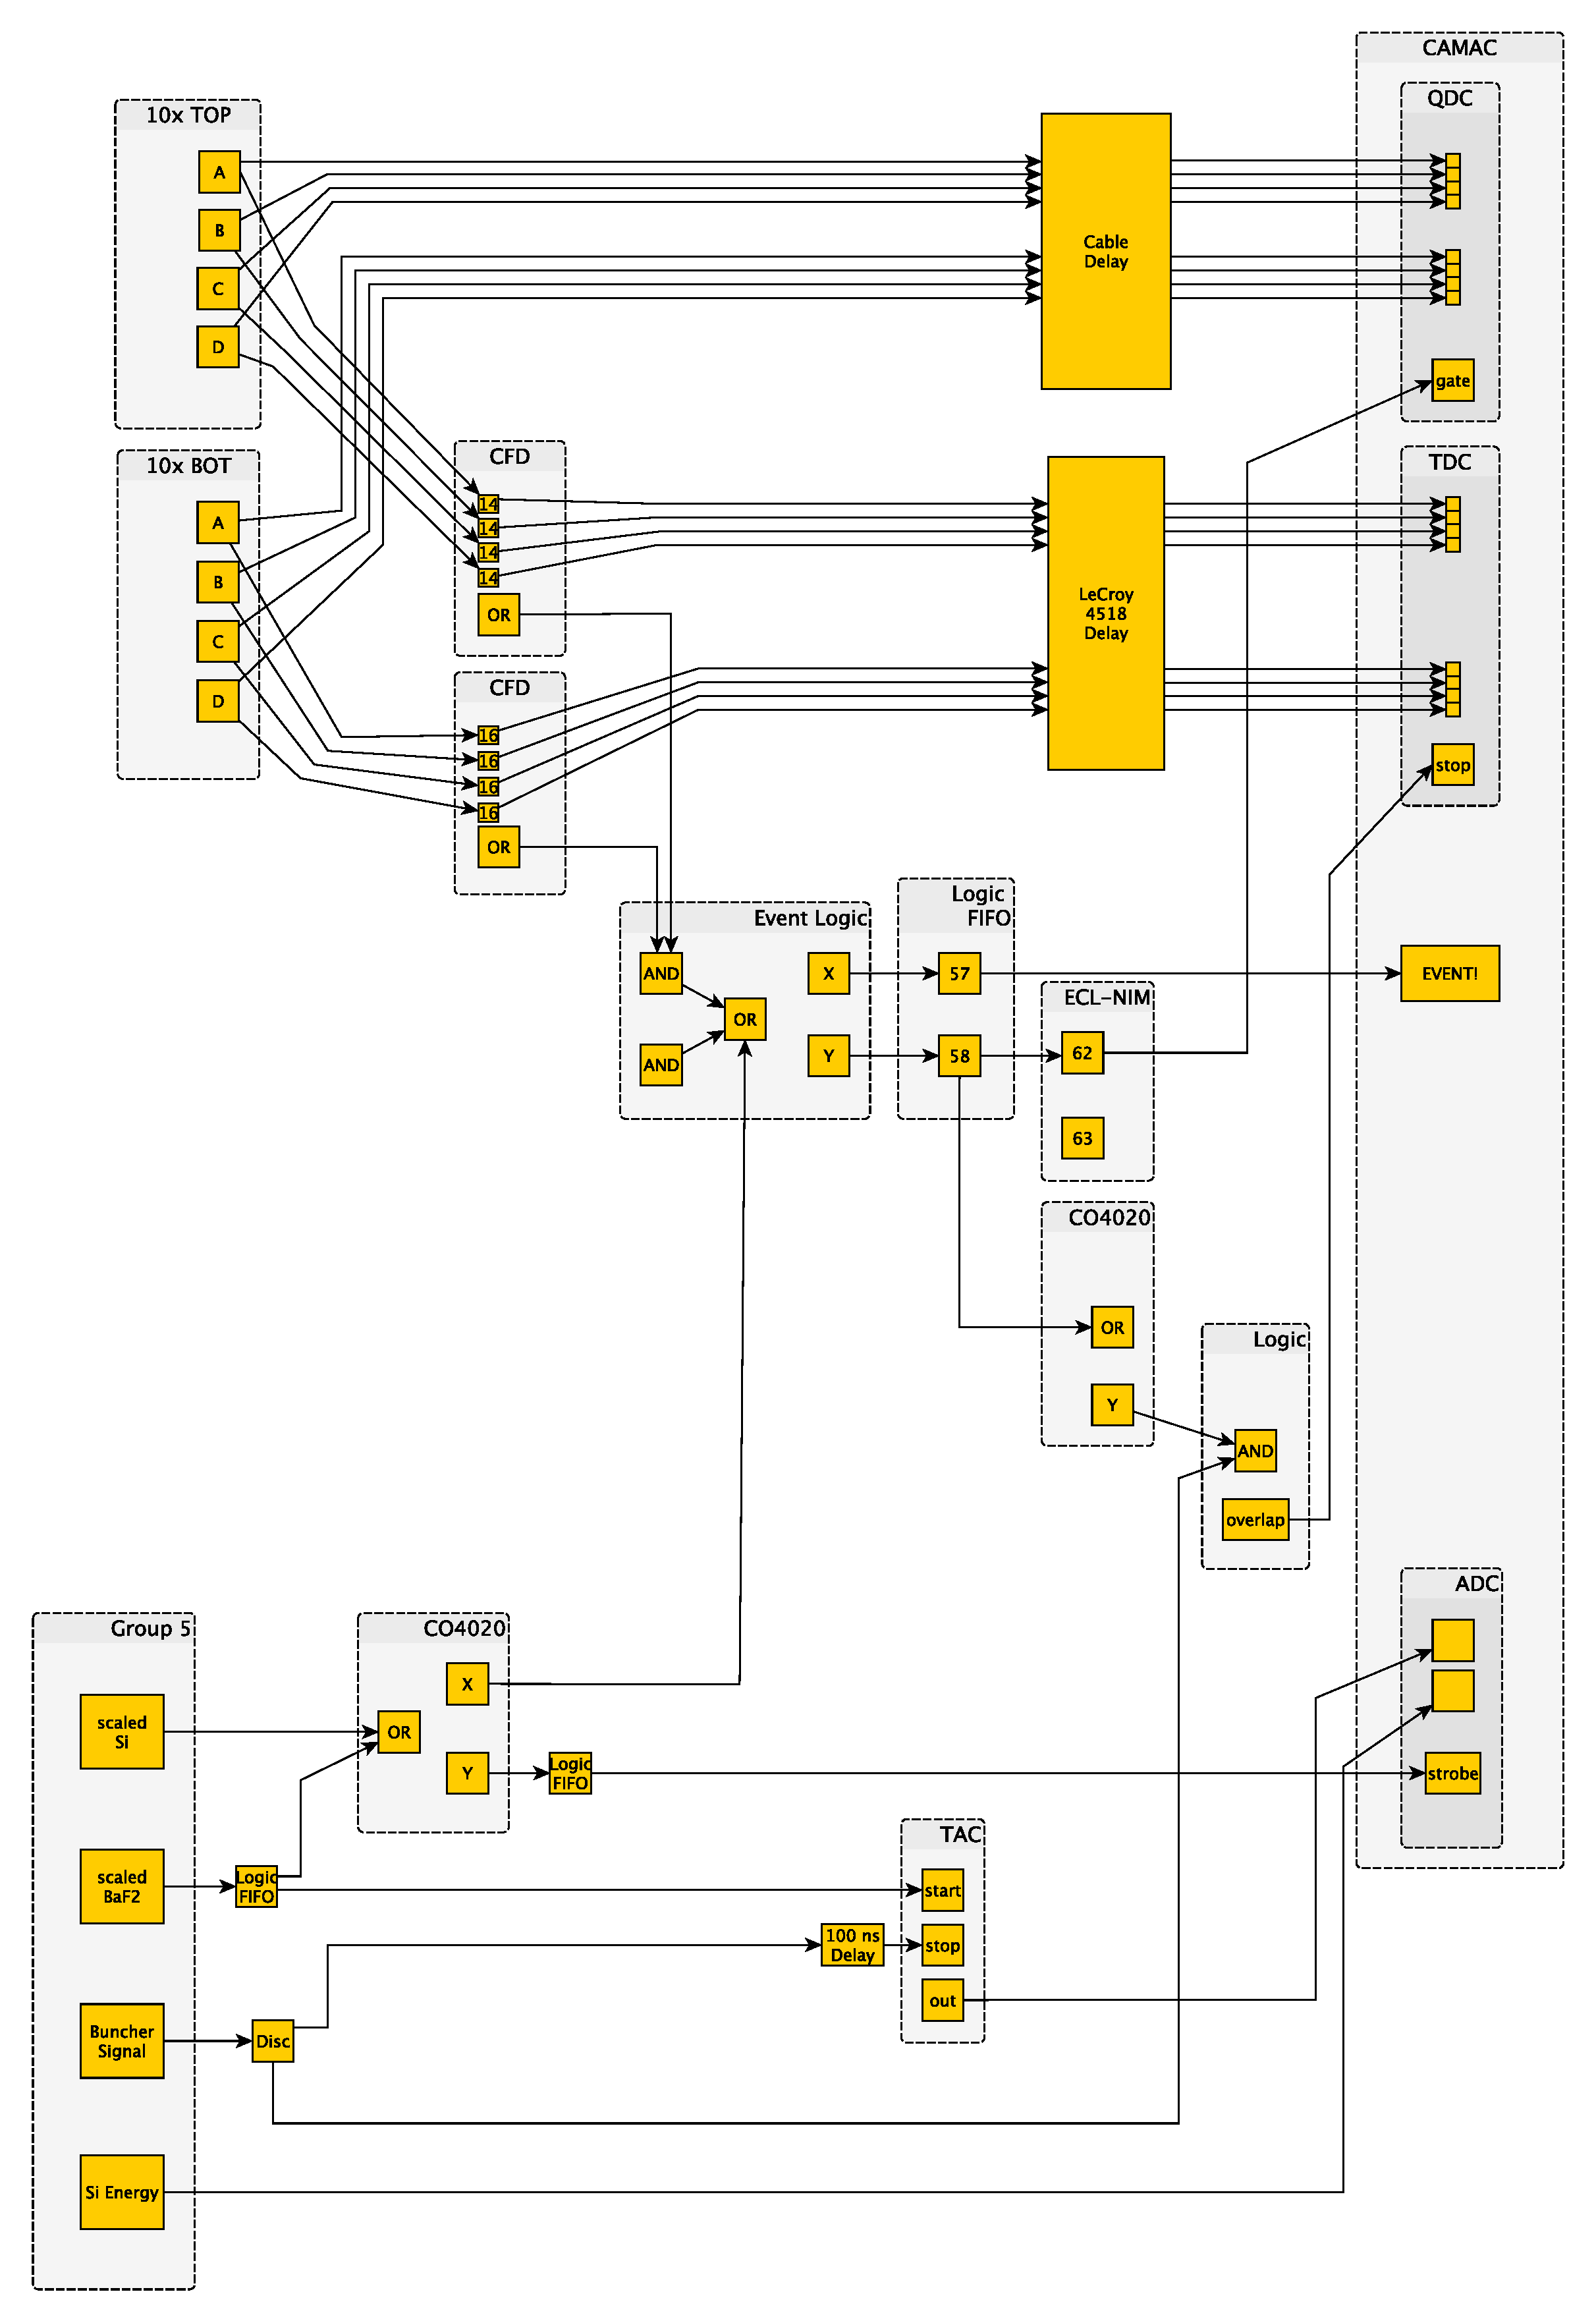
\includegraphics[height=0.8\textheight]{figures/electronics.eps}
\caption[Full diagram of the detector electronics.]{A diagram of the neutron detector electronics.  The modules on the right are read by the DAQ.}
\label{fig:fullElectronics}
\end{figure}

The DAQ must also record some quantities that are independent of the event trigger, such as the charge on the Faraday cup, which is needed to normalize the number of particles incident on the target between runs.  The DAQ records these as scalers.  {\fig}~\ref{fig:scalerElectronics} shows all the scalers that are recorded; many of these, such as the detector rates, are used only for monitoring during the run.  However, the live time and the charge are both used in the analysis.  The live scalers are important to record because the DAQ cannot collect new events while it is processing an event, and it is the live integrated beam current that is appropriate for cross-section calculations.  Measuring the live version of any scaler is possible using the busy signal the DAQ itself provides.  The busy signal is a NIM logic pulse that is low when the DAQ is busy.  Vetoing any scaler signal with this busy signal gives the live scaler, which is recorded in addition to the un-vetoed scaler.  The schematic is shown in {\fig}~\ref{fig:scalerElectronics}.  To turn the charge collected on the Faraday cup into a NIM signal that is compatible with the DAQ scaler, the Faraday cup is connected to a module that outputs a NIM logic pulse at a frequency that is proportional to the input charge.  This signal, like all the others, is recorded in both its raw and vetoed form.
% figure: Si, Q.live, NaI accumulation
% figure: full electronics
\begin{figure}[htp]
\centering
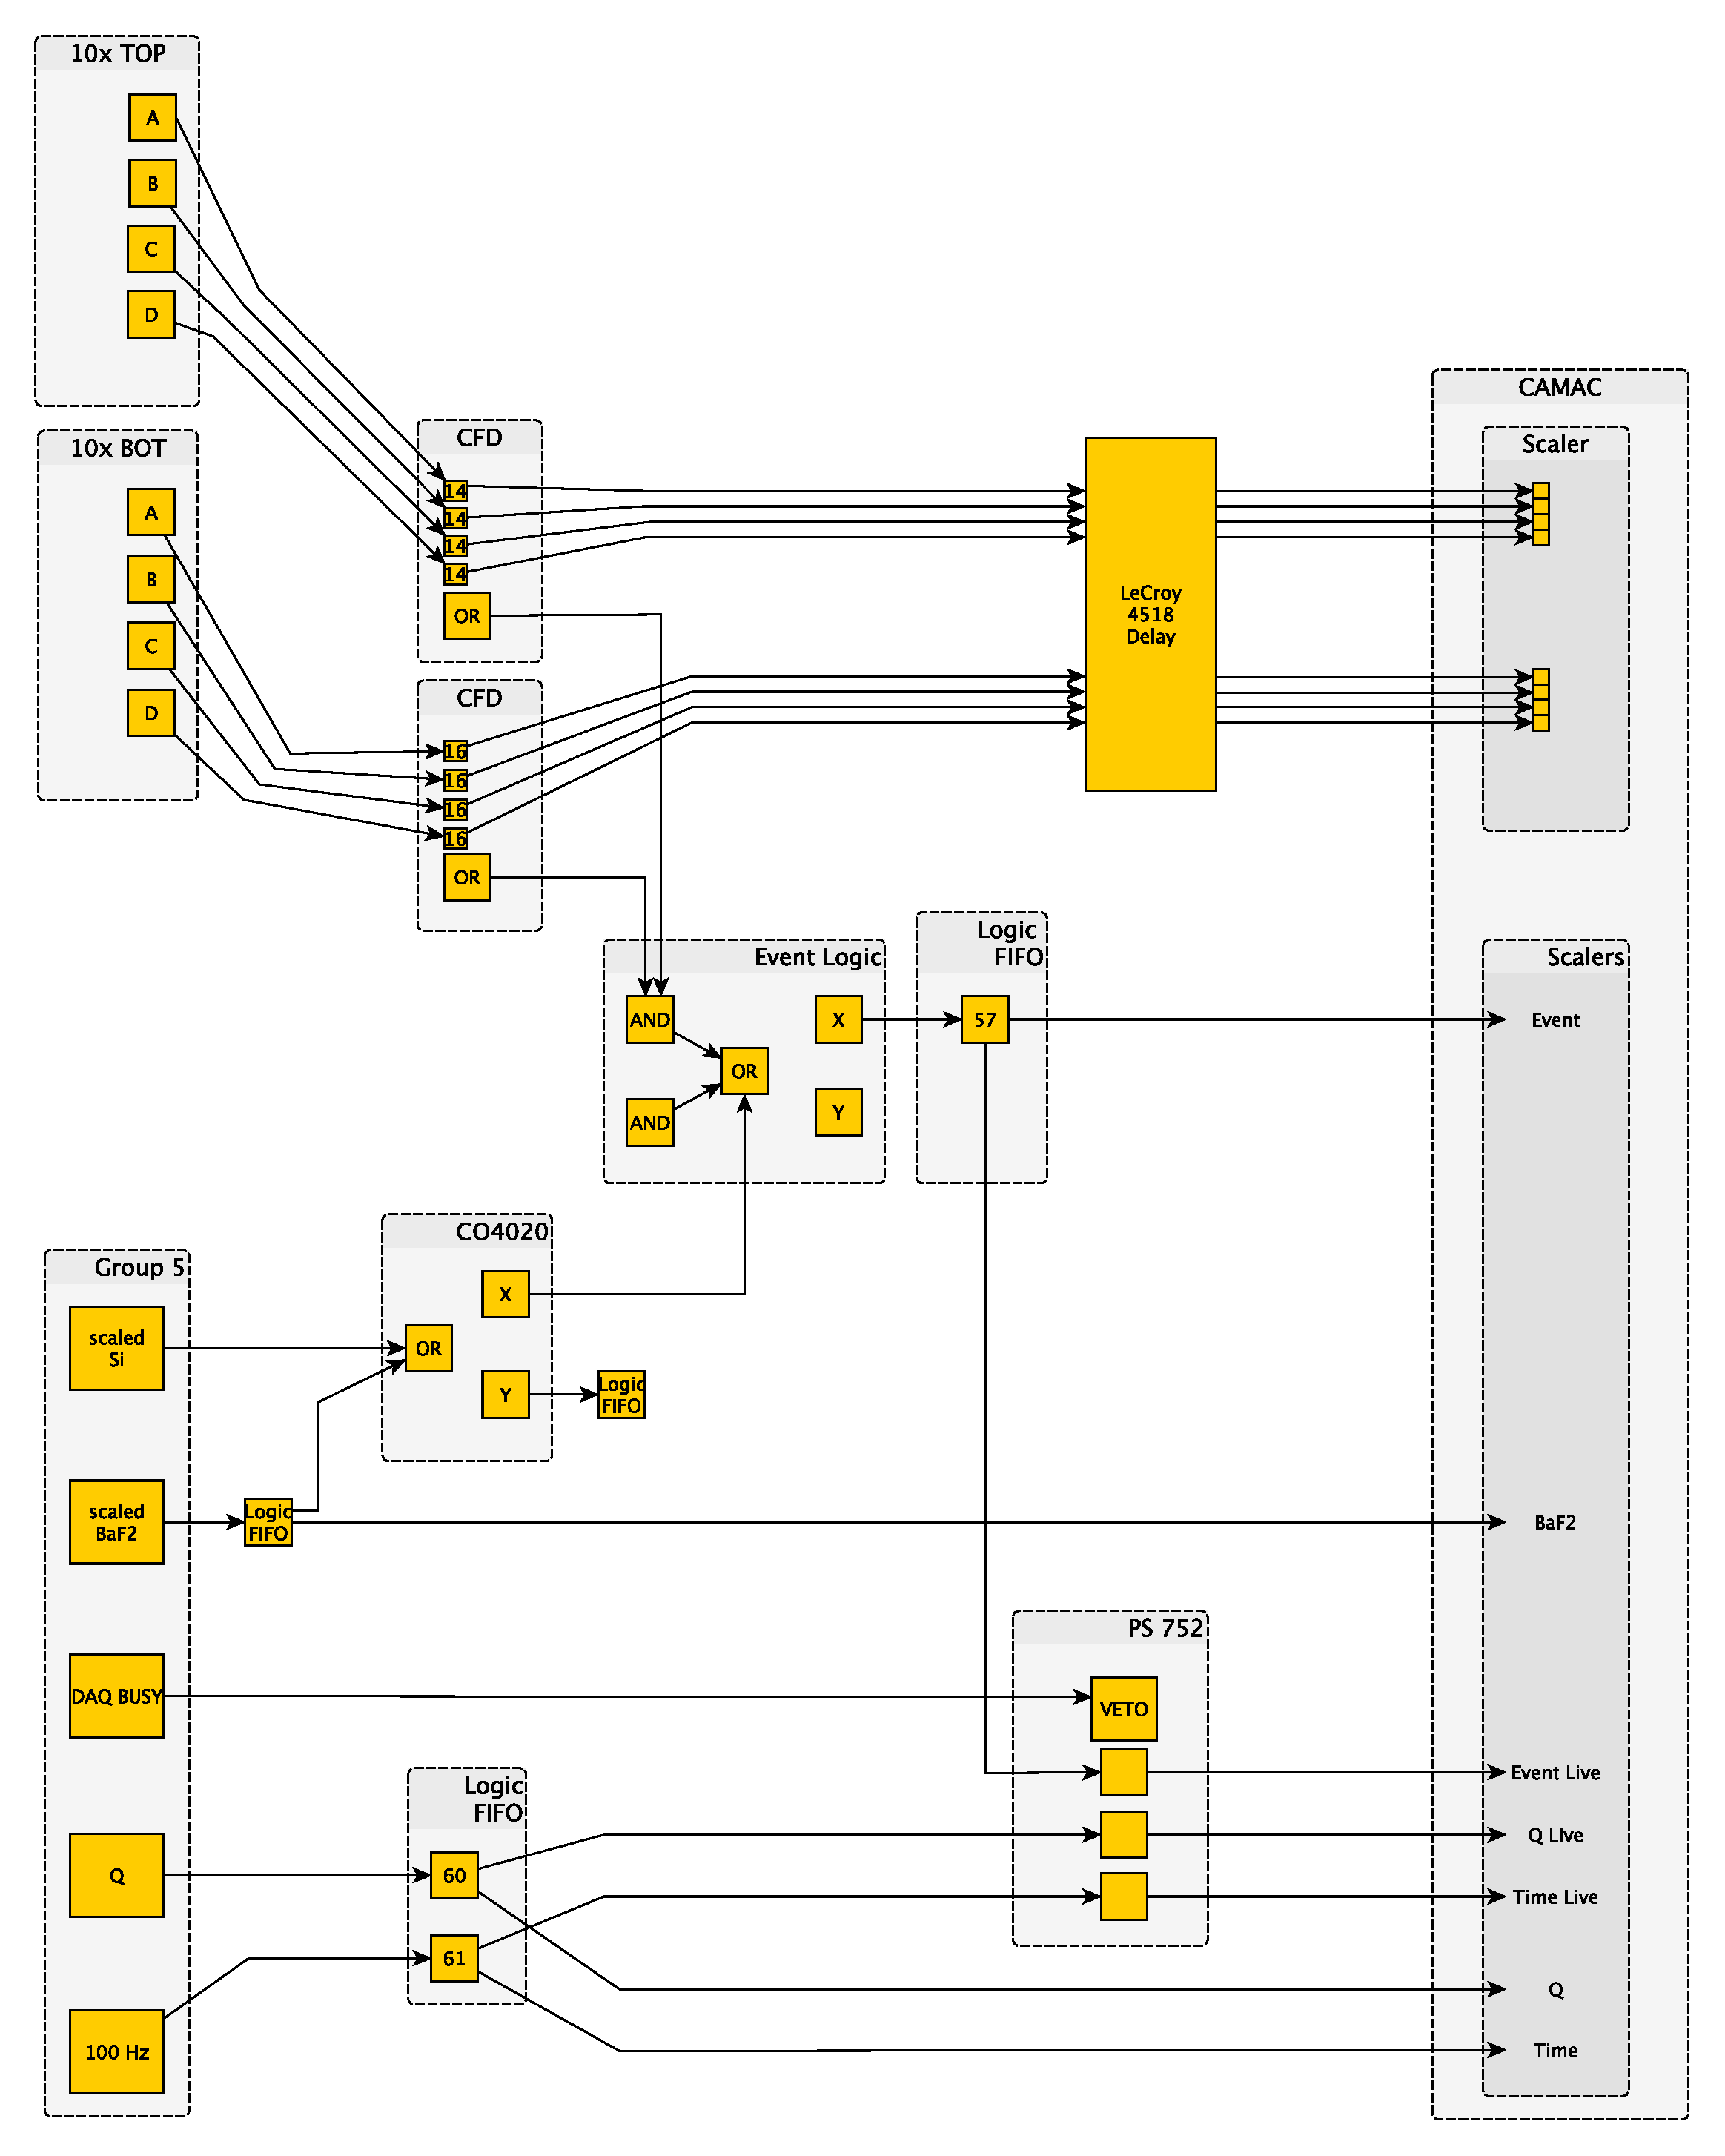
\includegraphics[height=0.8\textheight]{figures/electronics_scalers.eps}
\caption[Detector scalers.]{A diagram of the neutron detector scalers.  The modules on the right are read by the DAQ independent of the event signal.}
\label{fig:scalerElectronics}
\end{figure}
A test of this electronics setup using a \Mg{26} target verified the expected DAQ operation.  This test is discussed in the next chapter. 

% % uncomment the following lines,
% if using chapter-wise bibliography
%
% \bibliographystyle{ndnatbib}
% \bibliography{example}
